\chapter{Materials and methodologies}
In this section there's going to be an explanation of the dataset as well as instruments and methodologies used to analyze it's properties, as such the first step is going to be an in depth discussion of the data available and a general overview of the final use. The following step is going to be a description of the preliminary work done to the data itself and to the results of this preliminary analysis in order to select the important features. The final step of this chapter is going to be an explanation of the methods used to derive the final results and to evaluate them.

\section{Data and objective}
\label{chap:freefree}
The objective of this thesis is to find how different models for survival or clinical outcome behave as the input feature change. In other words a first part is the development of one or more models for survival analysis followed by a sensitivity analysis study of the developed models. The main focus is going to be on clinical images, i.e. lung CTs, used in conjunction with clinical and laboratory labels which are obtainable as soon as the patient is admitted in the hospital facilities. All clinical images are going to be analysed through the lens of \textbf{radiomics} while all clinical labels are provided as is by clinical professionals.
All images are non segmented, as such all of them are going to be semi-automatically segmented via a new software being tested in the medical physics department called \textit{\textbf{Sophia}}, which will be briefly explained shortly. Statistical analysis are going to be performed mainly in python using libraries such as scikit-learn, pandas, numpy, scipy while the graphical part of the analysis is done with either seaborn or matplotlib. \large{For the sake of time and simplicity some analysis was carried out in R language using the following libraries..... NON ANCORA MA SE SUCCEDE E' PRONTO DA AGGIUNGERE}
The starting dataset was a list of all the patients that, from 02/2020 to 05/2021, were hospitalized as COVID-19 positive inside the facilities of \textit{Azienda ospedaliero-universitaria di Bologna - Policlinico Sant'Orsola-Malpighi}. As far as exclusion criteria go the main exclusion criteria, except unavailability of the feature related to the patient, was visibly damaged or lower quality images, for example images with cropped lungs. The first set of selection criteria were:

\begin{itemize}
\item All patients that had undergone a CT exam which was retrievable via the PACS system of \textit{Azienda ospedaliero-universitaria di Bologna - Policlinico Sant'Orsola-Malpighi}
\item All patients that had a all of the clinical and laboratory features, listed in fig:\ref{fig:ClinicalFeatures}, suggested by Lidia Strigari \footnote{She is, as of the writing of this thesis, the head of the Medical Physics department in the S. Orsola hospital. These suggestions were given to her by clinical professionals.}
\item Since all patient had at least 2 CT exams only the closest date to the hospital admission date was taken. When more exams were performed on the same date all of them were initially taken. At first only chest or abdomen CTs were taken regardless of the acquisition protocol used.
\end{itemize}

\begin{figure}[H]
  		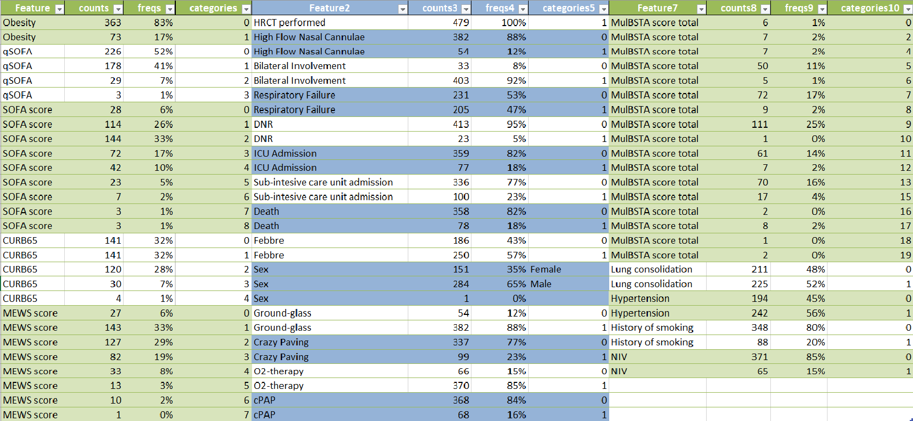
\includegraphics[width=1\textwidth]{Clinical_Feature_Description.png}
        \caption{Description of clinical label dataset, in sets of four columns there's the clinical feature, the total count of occurences, the percentage over the final dataset and the possible values the feature could take \label{fig:ClinicalFeatures}}
\end{figure}

Most clinical features are pretty self-explanatory, for those that were obscure to me as an outsider and not otherwise explained in \ref{Clinical_Covid_Manifestations}, I'm going to provide a very simple explanation:

\begin{enumerate}
\item DNR : Acronym for "Do Not Resuscitate", used to indicate the wish of the patient or their relatives that cardiac massage not be performed in case of cardiac arrest. 
\item NIV: Acronym for "Non Invasive Ventilation", it's a form of respiratory aid provided to patients.
\item cPAP: Acronym for  "continuous Positive Airway Pressure", another form of respiratory aid.
\item ICU: Acronym for "Intensive Care Unit". When patients are in really severe conditions they are treated in these facilities.
\item Clinical Scores: When available values from laboratory analyses and/or patient conditions are summarised in scores that represent the gravity of the state of the patient, as such these can be somewhat correlated and will be treated as comprehensive values to substitute an otherwise large set of obscure clinical features. At admission, or closely thereafter, a set of clinical questions regarding the patient receives a yes or no answer, each answer has an additive contribution towards the final value of the score.These scores differ in how much they add for each condition and the set of symptoms the check for.
	\begin{enumerate}
		\item MulBSTA: This score acconts for \textbf{Mul}tilobe lung involvement, absolute \textbf{L}ymphocyte count, \textbf{B}acterial coinfection, hystory of \textbf{S}moking, history of hyper\textbf{T}ension and \textbf{A}ge over 60 yrs. \cite{MulBSTA}
		\item MEWS: Modified Early Warning Score for clinical deterioration. Computed considering systolic blood pressure, heart rate, respiratory rate, temperature and AVPU(Alert Voice Pain Unresponsive) score. \cite{MEWS}
		\item CURB65: \textbf{C}onfusion, blood \textbf{U}rea Nitrogen or Urea level, \textbf{R}espiratory Rate, \textbf{B}lood pressure, age over \textbf{65} years. This score is specific for pneumonia severity \cite{CURB65}
		\item SOFA:  \textbf{S}equential  \textbf{O}rgan  \textbf{F}ailure  \textbf{A}ssessment score. Considers various quantities from all systems to assess the overall state of the patient, PaO$\_2$/FiO$\_2$\footnote{Very unrefined yet widely used indicator for lung disfunction} for respiratory system, Glasgow Coma scale\footnote{GCS for short, proposed in 1974 by Graham Teasdale and Bryan Jennet. Evaluates what kind of stymulus is necessary to obtain motor and verbal reactions in the patient as well as what's necessary for the patient to open their eyes} for nervous, mean pressure for cardiovascular, Bilirubin levels for liver, platelets for coagulation and creatine for kidneys \cite{SOFA}
		\item qSOFA:  \textbf{q}uick SOFA. Only considers pressure, high respiratory rate and the low values in the Glasgow scale.
	\end{enumerate}	
\end{enumerate}

This procedure produced a starting cohort of $\sim$700 patients which, having all various images available, created a huge set of $\sim$2200 CT scans. Since this analysis is focused on radiomics there is an evident need for as much consistency as possible in the images analysed. For this reason all CTs taken with medium of contrast were excluded, since they would have brightnesses not justified, and for every patient only images with thin slice reconstruction were considered. More specifically only images with slice thickness of 1 o 1.25 mm\footnote{This meant that only exams called 'Parenchima' or  'HRCT' were included. Throughout the internship 'parenchima' has always appeared in contrast with 'mediastino'. These two keywords are used in the phase of reconstruction of the raw data to identify reconstructions with specific properties. Parenchima is used for finer reconstruction of lung specifically, the requiring professional uses these images to look for small nodules with very high contrast and, to do so, the reconstruction allows some noise to achieve the best resolution possible. Mediastino is used in the lung, as well as other regions, to look for bigger lesions but with low contrast. As such the 'mediastino' reconstruction compromises a worse spatial resolution for a better display of contrast, visually speaking the first images are more coarse and noisy while the second are smoother. It should be noted that even with the same identifier, be it HRCT parenchima or others, the machines on which the exams were made were different and had different proprietary convolutional kernels used for reconstruction.} along the z-axis were taken into consideration, which meant excluding all the 1.5,2,2.5 and 5 mm slice thicknesses.
Since all these images were segmented by me and two other students using a semiautomatic segmentation tool provided by the hospital it sometimes happened that manual corrections were necessary, these were performed only in very obvious and simple cases while, in all remaining cases, the patient was dropped out of the study. 
Overall this left the final study cohort to be composed of 436 patients, all descriptions and analyses are related to this cohort.





























